\documentclass[12pt,a4paper]{report}
\usepackage{graphicx}
\usepackage{hyperref}
\usepackage{amsmath}
\usepackage{listings}
\usepackage{float}
\usepackage{color}
\usepackage{xcolor}
\usepackage{geometry}
\geometry{margin=1in}

% Define custom colors
\definecolor{codegray}{rgb}{0.5,0.5,0.5}
\definecolor{codepurple}{rgb}{0.58,0,0.82}
\definecolor{backcolour}{rgb}{0.95,0.95,0.92}
\definecolor{headercolor}{rgb}{0.1,0.3,0.6}
\definecolor{sectioncolor}{rgb}{0.2,0.5,0.8}

\lstdefinestyle{mystyle}{
    backgroundcolor=\color{backcolour},
    commentstyle=\color{codegray},
    keywordstyle=\color{blue},
    numberstyle=\tiny\color{codegray},
    stringstyle=\color{codepurple},
    basicstyle=\ttfamily\footnotesize,
    breakatwhitespace=false,
    breaklines=true,
    captionpos=b,
    keepspaces=true,
    numbers=left,
    numbersep=5pt,
    showspaces=false,
    showstringspaces=false,
    showtabs=false,
    tabsize=2
}

\lstset{style=mystyle}

% Define custom title style
\title{\color{headercolor}\textbf{Blockchain Project Report}}
\author{Your Team Name}
\date{\today}

\begin{document}

\maketitle

\hypersetup{
    colorlinks=true,
    linkcolor=headercolor,
    urlcolor=sectioncolor,
    pdftitle={Blockchain Project Report},
    pdfpagemode=FullScreen,
}

% Enhanced Table of Contents
\renewcommand{\contentsname}{\color{headercolor}\textbf{Table of Contents}}
\tableofcontents

\chapter{Introduction to Blockchain}
\section{Motivation and Basic Definitions}
A blockchain is a distributed database that maintains a continuously growing list of records, called blocks, secured from tampering and revision.

\section{Encryption}
\subsection{Functions}
Encryption functions transform plaintext into ciphertext, ensuring confidentiality.
\subsection{Symmetric-Key Algorithm}
Symmetric algorithms use the same key for encryption and decryption.
\subsection{Asymmetric-Key Algorithm}
Asymmetric algorithms use a public-private key pair for secure communication.

\section{Hashing}
Hashing ensures data integrity by converting input into fixed-size hash values.

\section{Smart Contracts}
Smart contracts are self-executing contracts with the agreement terms directly written into code.

\section{Bitcoin}
Bitcoin was the first implementation of blockchain technology, allowing decentralized transactions.

\section{Example Workflows}
Example workflows include transaction creation, mining, and verification processes.

\section{Summary}
Blockchain introduces trustless, decentralized systems to enhance security and transparency.


\chapter{UML Diagrams}
\section{Class Diagram}
\includegraphics[width=\textwidth]{path/to/class_diagram.png}

\section{Use Case Diagram}
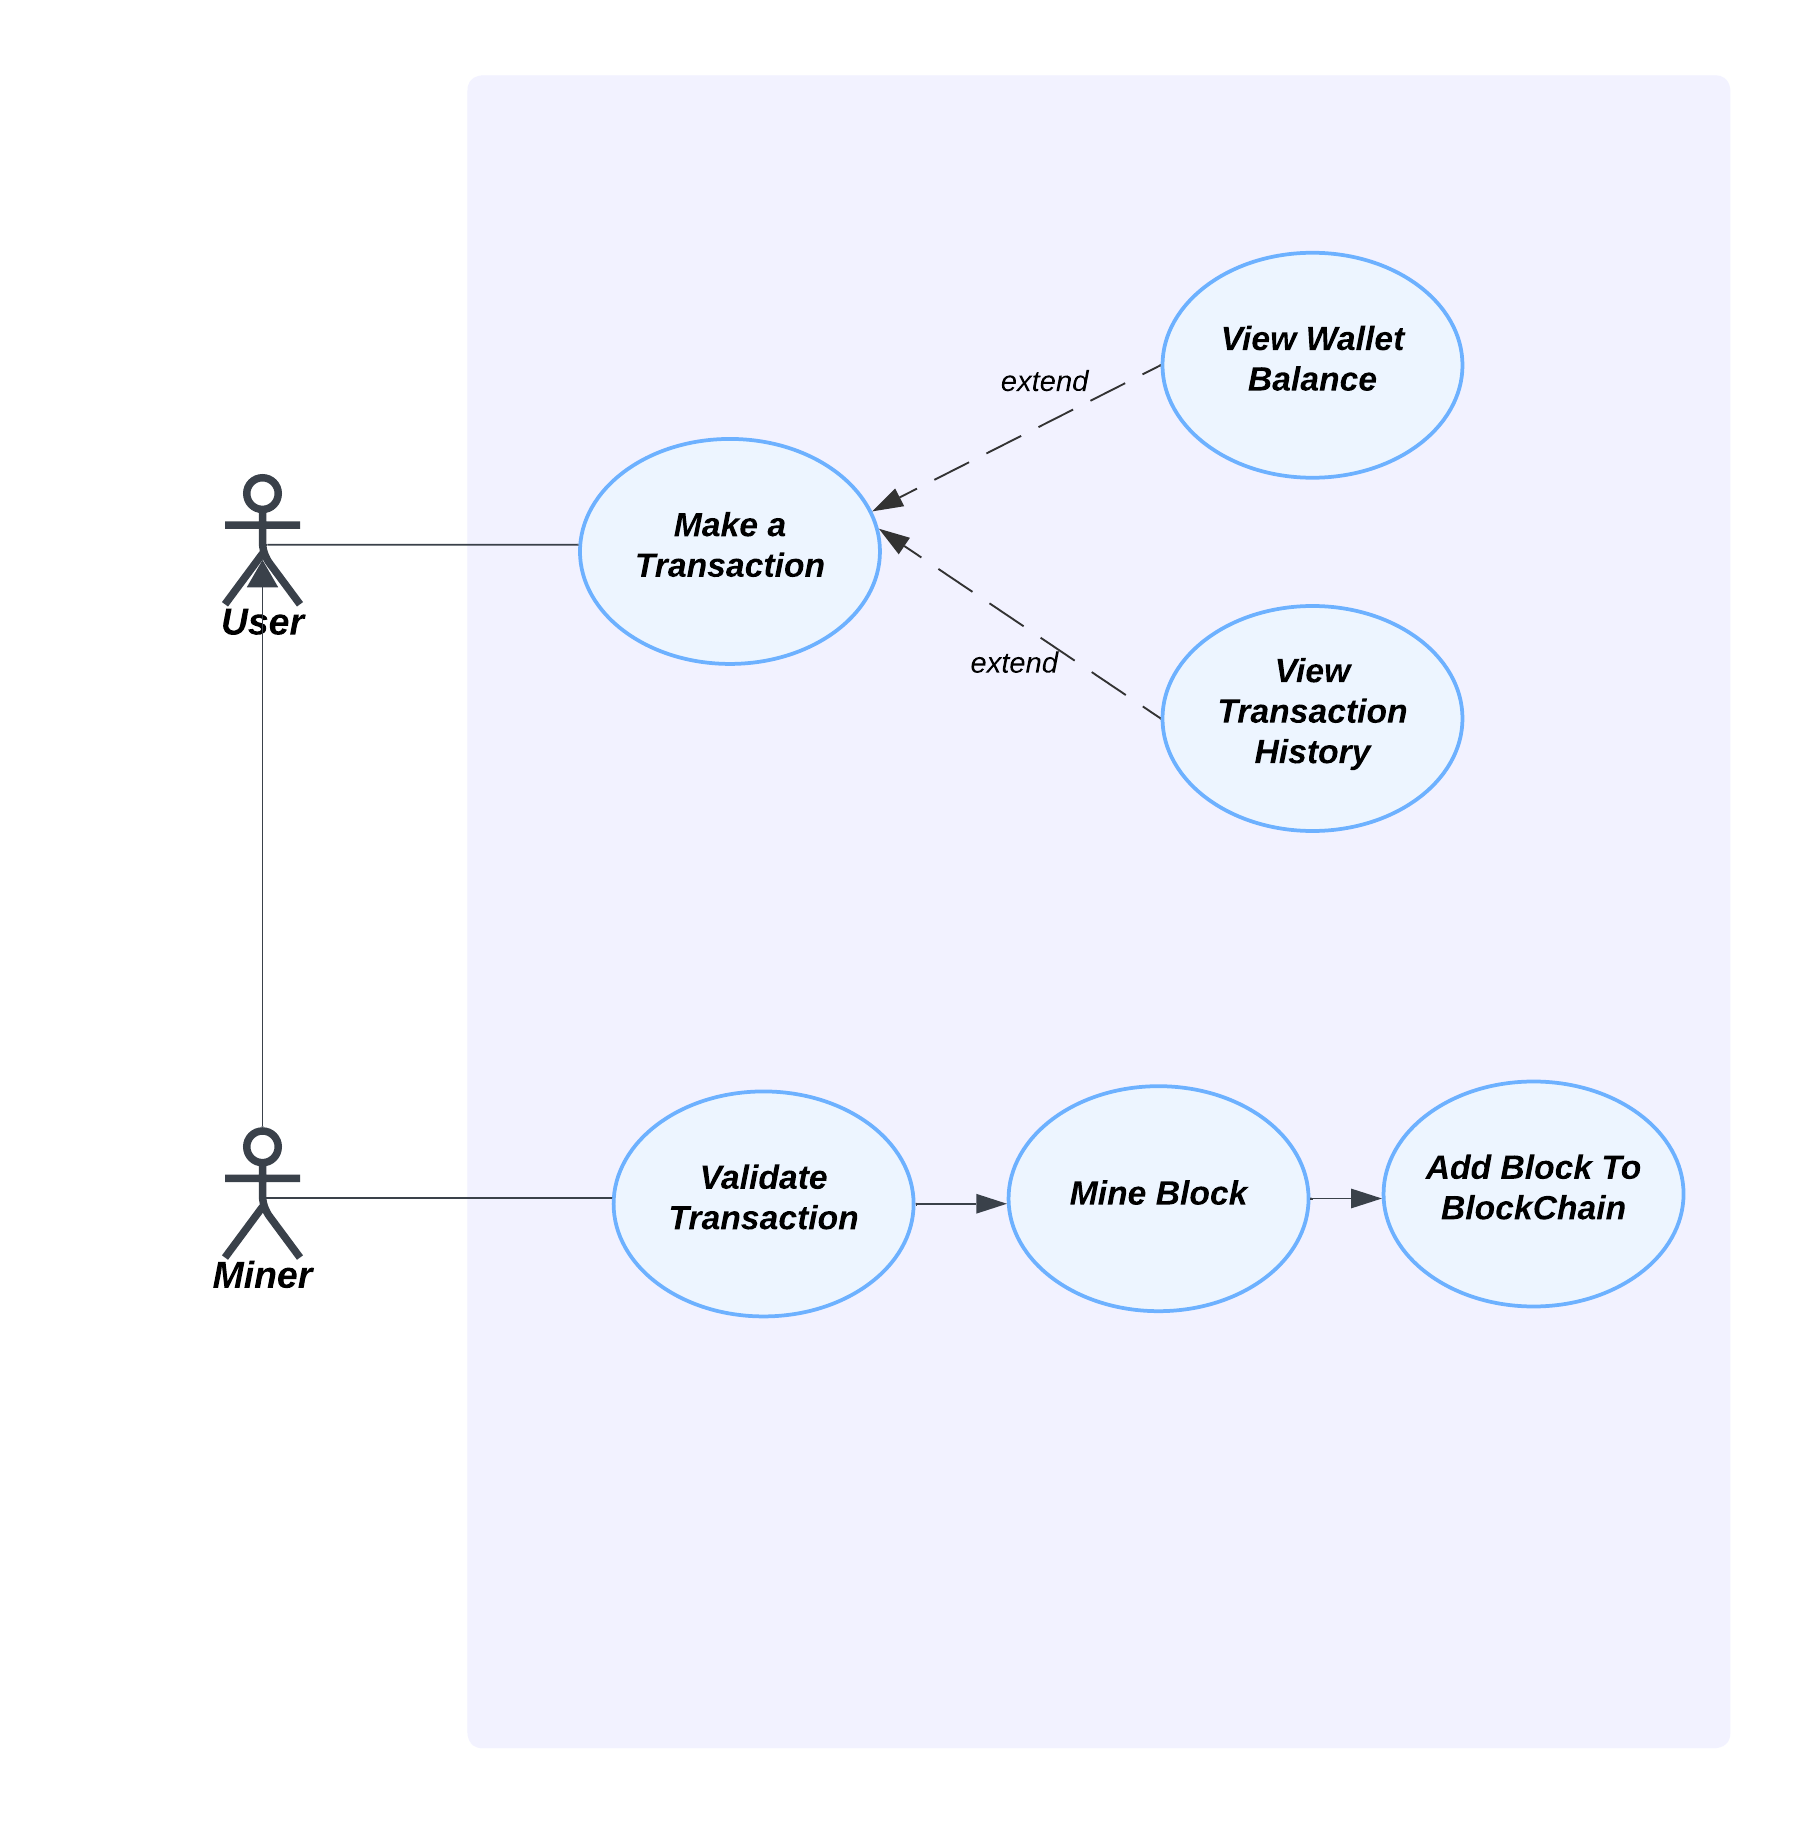
\includegraphics[width=\textwidth]{usecasesdiagram.png}
\textbf{User Processes}
\begin{enumerate}
    \item Make a Transaction:
        \begin{itemize}
        \item A user initiates a transaction by providing the necessary details.
        \item This step is the primary action a user takes when interacting with the blockchain.
        \end{itemize}
    
    \item View Wallet Balance (Extension):
        \begin{itemize}
        \item The user can check their current wallet balance.
        \item This functionality provides transparency and ensures that the user has sufficient funds for the transaction
        \end{itemize}
        
     \item View Transaction History (Extension):
        \begin{itemize}
        \item The user can review past transactions recorded on the blockchain.
        \item This offers a way to verify the history of operations and ensure accountability.
        \end{itemize}
\end{enumerate}
\textbf{Miner Processes}
\begin{enumerate}
    \item Validate Transaction:
        \begin{itemize}
        \item The miner checks the transaction's validity.
        \item This involves verifying the sender's signature, ensuring the wallet has sufficient funds, and confirming that the transaction adheres to the blockchain's rules.
        \end{itemize}
    
    \item Mine Block:
        \begin{itemize}
        \item After validating transactions, the miner groups them into a block.
        \end{itemize}
        
    \item Add Block to Blockchain:
        \begin{itemize}
        \item The miner adds the newly created block to the blockchain.
        \item This ensures the transaction is permanently recorded.
        \end{itemize}
\end{enumerate}
\textbf{End-to-End Workflow}


\begin{enumerate}
    \item User Interaction:
        \begin{itemize}
        \item A user initiates a transaction and, optionally, checks their wallet balance or transaction history for transparency.
        \end{itemize}
    
    \item Transaction Validation:
        \begin{itemize}
        \item Miners verify the transaction to ensure it is legitimate and secure.
        \end{itemize}
        
    \item Block Mining:
        \begin{itemize}
        \item Valid transactions are grouped into a block.
        \end{itemize}

    \item Updating the Blockchain:
        \begin{itemize}
        \item Once mined, the block is added to the blockchain, making the transaction permanent.
        \end{itemize}
\end{enumerate}





\section{Sequence Diagram}
\includegraphics[width=\textwidth]{path/to/sequence_diagram.png}


\chapter{Model: Blockchain Core}


\section{Block.java}
\paragraph{}
We will start first by listing the imports in the following code snippet:
\begin{lstlisting}[language=Java]
package com.blockchain.model;

import com.google.gson.Gson;
import lombok.Getter;
import lombok.Setter;

import java.security.*;
import java.security.spec.InvalidKeySpecException;
import java.security.spec.X509EncodedKeySpec;
import java.util.ArrayList;
import java.util.Arrays;
import java.util.LinkedList;
import java.util.List;
\end{lstlisting}
\paragraph{}
Next we move on to our class declaration and fields, as shown in our next code snippet:

\begin{lstlisting}[language=Java]
public class Block {

    private byte[] prevHash;
    private byte[] currHash;    
    private String timeStamp; 
    private byte[] minedBy;
    private Integer ledgerId = 1;
    private Integer miningPoints = 0;
    private Double luck = 0.0;

    private List<Transaction> transactionLedger = new ArrayList<>();
\end{lstlisting}
\paragraph{}
Since all the blocks for our blockchain will be created using this class, we need them to be serializable so that we can share our blockchain through our network.
The field prevHash will contain the signature or, in other words, the encrypted data from the previous block. The currHash will contain the signature or, in other words, the encrypted data from this block, which will be encrypted with the private key of the miner that will get to mine this block. The timeStamp obviously will contain a timestamp of when this block was mined/finalized. The field minedBy will contain the public key, which also doubles as the public address of the miner that managed to mine this block. In the process of blockchain verification, this public address/public key will be used to verify that the currHash/signature of this block is the same as the hash of the data presented by this block and secondary that this block was indeed mined by this particular miner. 
 We will touch on this topic a bit later in this section when we explain the isVerified method of this class. Next is our ledgerId field. Since we intend to implement a database with separate Block and Transaction tables, this field will help us retrieve the correct corresponding ledger for this block. You can also look at this field as the block number. Our next fields, miningPoints and luck, will be used to form the network consensus in regard to choosing this block’s miner.
We will get into the details of how these fields are used in \hyperref[chapter Service Layer]{Chapter 7}. The field transactionLedger is simply an arraylist of all the transactions contained in this block. We will explain the Transaction class in the section “Transaction.java.”
\paragraph{}
In the following snippet, we can see the three constructors:
\begin{lstlisting}[language=Java]
    public Block(byte[] prevHash, byte[] currHash, String timeStamp, byte[] minedBy, Integer ledgerId,
            Integer miningPoints, Double luck, List<Transaction> transactionLedger) {
        this.prevHash = prevHash;
        this.currHash = currHash;
        this.timeStamp = timeStamp;
        this.minedBy = minedBy;
        this.ledgerId = ledgerId;
        this.miningPoints = miningPoints;
        this.luck = luck;
        this.transactionLedger = transactionLedger;
    }

    public Block(LinkedList<Block> currentBlockChain) {
        Block lastBlock = currentBlockChain.getLast();
        prevHash = lastBlock.getCurrHash();
        ledgerId = lastBlock.getLedgerId() + 1;
        luck = Math.random() * 1000000;
    }

    public Block() {
        prevHash = new byte[] { 0 }; // initiate the array with zeros
    }
\end{lstlisting}
\paragraph{}
The first constructor is used when we retrieve our blockchain from 
the database. Here we retrieve all the blocks completely finalized, and this 
constructor helps us instantiate the block with all of the fields properly 
set up. The second constructor is used while the application is running 
and is used to create a completely new block (in other words, the head of 
the blockchain) for us to work on. We will go over the details of how this is 
achieved in \hyperref[chapter Service Layer]{Chapter 7}. Our third constructor on line 20 will be used only once by our init() method to create our first block.
\paragraph{}
Our next snippet showcases the isVerified method:
\begin{lstlisting}[language=Java]
    public Boolean isVerified(Signature signing)throws InvalidKeyException, SignatureException, NoSuchAlgorithmException, InvalidKeySpecException {

        X509EncodedKeySpec keySpec = new X509EncodedKeySpec(this.minedBy);
        KeyFactory keyFactory = KeyFactory.getInstance("DSA");
        PublicKey publicKey = keyFactory.generatePublic(keySpec);

        // Initialize the Signature with the PublicKey for verification
        signing.initVerify(publicKey);

        // Generate a hash of the block's data (excluding the currHash, which is the
        // signature)
        byte[] blockDataHash = this.toString().getBytes(); // Use relevant block data to hash

        // Update the Signature with the data to verify (usually the block data or hash)
        signing.update(blockDataHash);

        // Verify the signature with the current hash
        return signing.verify(this.currHash);
    }
\end{lstlisting}
\paragraph{}
We accept an object from the Signature class as a parameter. The Signature class is actually a class from the java security package java.security.Signature. It is a helper singleton class that allows us to encrypt/decrypt data using different algorithms. On line 8 we verify the data in this class against the signature stored in the currHash. On line 15 we insert the data that we want to verify. On line 18 we return the Boolean result after verifying the data contained in this class against its currHash.
\paragraph{}
What’s left, as shown in our next snippet, are the equals and hash methods, the toString() method,the toJson() method ,which concludes our Block.java class:
\begin{lstlisting}[language=Java]
    public boolean equals(Object o) {
        if (this == o)
            return true;
        if (!(o instanceof Block block))
            return false;
        return Arrays.equals(getPrevHash(), block.getPrevHash());
    }

    @Override
    public int hashCode() {
        return Arrays.hashCode(getPrevHash());
    }

    @Override
    public String toString() {
        return "Block{" + "luck=" + luck + ", miningPoints=" + miningPoints + ", ledgerId=" + ledgerId + ", minedBy="
                + Arrays.toString(minedBy) + ", timeStamp='" + timeStamp + '\'' + ", prevHash="
                + Arrays.toString(prevHash) + '}';
    }

    public String toJson() {
        Gson gson = new Gson();
        return gson.toJson(this);
    }
\end{lstlisting}
\paragraph{}
The first thing to note here is that the equals method compares the previous hash of the block class. We’ll use this later in \hyperref[chapter Service Layer]{Chapter 7} when we explain the consensus algorithm further. The other thing of note is the fields contained in the toString method. We include everything that goes into verifying the block against the current hash.


 
\section{Transaction.java}
\paragraph{}
 We briefly mentioned that we keep an array list of transactions in our Block class in the previous section, and now it’s time to explain in detail what our Transaction.java class contains. First we’ll start with the imports found in the following code snippet:
 \paragraph{}
 
 
\begin{lstlisting}[language=Java]
package com.blockchain.model;

import com.google.gson.Gson;
import lombok.Getter;
import lombok.Setter;

import java.security.*;
import java.security.spec.InvalidKeySpecException;
import java.security.spec.X509EncodedKeySpec;
import java.time.LocalDateTime;
import java.util.Arrays;
import java.util.Base64;
\end{lstlisting}
\paragraph{}
Next let’s go over the class declaration and its fields, as shown in the next code snippet:
\paragraph{}

\begin{lstlisting}[language=Java]
public class Transaction {

    private byte[] from;
    private String fromFX;
    private byte[] to;
    private String toFX;
    private Integer value;
    private String timestamp;
    private byte[] signature;
    private String signatureFX;
    private Integer ledgerId;
\end{lstlisting}

\paragraph{}
The fields from and to will contain the public keys/addresses of the account that sends and the account that receives the coins, respectively. 
The value is the amount of coins that will be sent, and timeStamp is the time at which the transaction has occurred. Signature will contain the encrypted information of all the fields, and it will be used to verify the validity of the transaction (it will be used the same way the field currHash was used in the previous class).The ledgerId serves the same purpose as in the previous class. The fields with the FX suffix are simple duplicates formatted to String instead of byte[]. We do this so that we can easily display them on our front end.
In this class we also have two constructors; the first one is used when we retrieve a transaction from the database, and the second one is used when we want to create a new transaction within our application.Let’s observe them in the following code snippet:
\begin{lstlisting}[language=Java]
    public Transaction(
            byte[] from,
            byte[] to,
            Integer value,
            byte[] signature,
            Integer ledgerId,
            String timeStamp
    ) {
        Base64.Encoder encoder = Base64.getEncoder();
        this.from = from;
        this.fromFX = encoder.encodeToString(from);
        this.to = to;
        this.toFX = encoder.encodeToString(to);
        this.value = value;
        this.signature = signature;
        this.signatureFX = encoder.encodeToString(signature);
        this.ledgerId = ledgerId;
        this.timestamp = timeStamp;
    }


    /**
     * Constructor for creating a new transaction and signing it.
     * <br>
     * used when we want to create a new transaction within our application
     *
     * @param fromWallet the fromWallet parameter contains the public and
     *                   private keys of the sender/maker of the transaction.
     */
    public Transaction(
            Wallet fromWallet,
            byte[] toAddress,
            Integer value,
            Integer ledgerId,
            Signature signing
    ) throws InvalidKeyException, SignatureException {
        Base64.Encoder encoder = Base64.getEncoder();
        this.from = fromWallet.getPublicKey().getEncoded();
        this.fromFX = encoder.encodeToString(fromWallet.getPublicKey().getEncoded());
        this.to = toAddress;
        this.toFX = encoder.encodeToString(toAddress);
        this.value = value;
        this.ledgerId = ledgerId;
        this.timestamp = LocalDateTime.now().toString();
        signing.initSign(fromWallet.getPrivateKey());
        String sr = this.toString();
        signing.update(sr.getBytes());
        this.signature = signing.sign();
        this.signatureFX = encoder.encodeToString(this.signature);
    }

\end{lstlisting}

\paragraph{}
The first constructor simply sets the class fields according to the retrieved data from the database and uses the Base64.Encoder class to convert the byte[] fields safely into String.
The second constructor is a bit more complex, so we will explain it in more detail piece by piece. First let’s look at the constructor parameters that are different: Wallet fromWallet and Signature signing. We will explain the Wallet class in more detail in the next section, for now we should just note that the fromWallet parameter contains the public and private keys of the sender/maker of the transaction. We use the same Signature class as in our Block isVerified method mentioned in the previous section.
Next let’s explain the body of the constructor so we understand how encrypting data works in our case. The signature creation phase shown in Figure below offers an overview of what we are trying to accomplish.


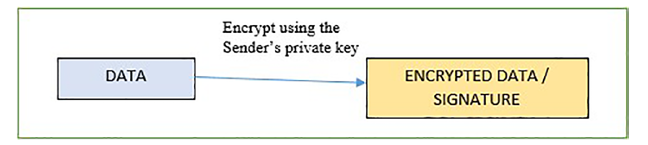
\includegraphics[width=\textwidth]{image.png}
\paragraph{}


To achieve this, first we set up our data by initiating our class fields from the parameters and add a timestamp as shown on lines 38 to 44. Now once we have our data that we would like to encrypt, we set our private key to the signing object with the statement on line 45. This tells the signing object, when encrypting, to use the private key we provided. On line 46 we are putting all the data we want to encrypt in a single String object by using the toString() method. On line 47 we are feeding all the data we want to encrypt to the signing object, and on line 48 we are actually encrypting the data and assigning it to our signature field.
Next is our method for the verification of transactions, as shown in the following snippet:
\paragraph{}


\begin{lstlisting}[language=Java]
public Boolean isVerified(Signature signing)
            throws InvalidKeyException, SignatureException, NoSuchAlgorithmException, InvalidKeySpecException {
        X509EncodedKeySpec keySpec = new X509EncodedKeySpec(getFrom());
        KeyFactory keyFactory = KeyFactory.getInstance("DSA");
        // public key of sender
        PublicKey publicKey = keyFactory.generatePublic(keySpec);

        signing.initVerify(publicKey);
        signing.update(this.toString().getBytes());
        return signing.verify(this.getSignature());
    }

\end{lstlisting}
\paragraph{}

This method will be used by the other peers to verify that each transaction is valid. Before explaining the code, let’s look at Figure below and see what our method tries to accomplish.


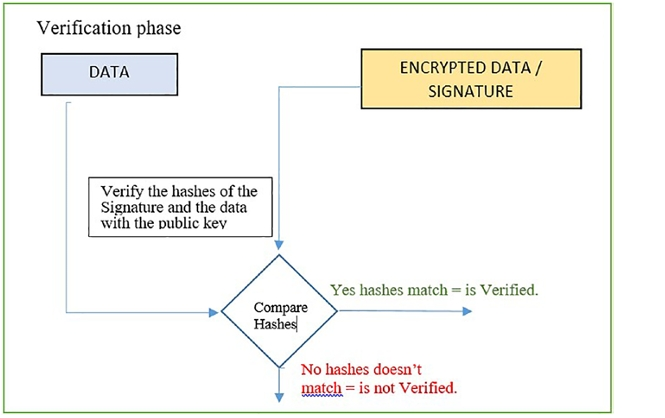
\includegraphics[width=\textwidth]{image2.jpeg}
\paragraph{}


The workflow of the schematic is quite simple; we need to compare the hash of the signature and the hash of the data contained in our class using the public key.
Now let’s look back at our isVerified method and explain how the workflow from the schematic is achieved. As parameters we are getting the Transaction object that we want to verify and the Signature helper class object, which pre-initialized to use SHA256 with DSA algorithm the same way as before. On line 8 we are setting the public key with which we would like to decrypt our signature. The new DSAPublicKeyImpl(byte[] encoded) is just a wrapper from the sun.security.provider package that will help convert our public key information from byte[] to PublicKey object. On line 9 we set the transaction data that we want to verify against the signature. Finally on line Blockchaintransaction.java 10 we provide the signature, the process of comparison/verification gets executed and a result is returned automatically for us.
We finish up the rest of the class with generic our toString, equals, toJson ,and hash methods, as shown in the following snippet:
\paragraph{}



\begin{lstlisting}[language=Java]
public String toString() {
        return "Transaction{" +
                "from=" + Arrays.toString(from) +
                ", to=" + Arrays.toString(to) +
                ", value=" + value +
                ", timeStamp= " + timestamp +
                ", ledgerId=" + ledgerId +
                '}';
    }


    /**
     * two Transactions are equal if and only if they have the same signature
     * <br>
     * signature is used because we're certain it's unique.
     * {@link #timestamp} proves the uniqueness of the Transaction
     */
    @Override
    public boolean equals(Object o) {
        if (this == o) return true;
        if (!(o instanceof Transaction that)) return false;
        return Arrays.equals(getSignature(), that.getSignature());
    }

    @Override
    public int hashCode() {
        return Arrays.hashCode(getSignature());
    }

    /**
     * Converts the current Transaction object to a JSON string.
     * @return JSON representation of the Transaction object.
     */
    public String toJson() {
        Gson gson = new Gson();
        return gson.toJson(this);
    }

\end{lstlisting}





\section{Wallet.java}
\paragraph{}
Let’s start as always with the imports for this class located in the following 
snippet:

\begin{lstlisting}[language=Java]
package com.blockchain.model;

import com.google.gson.Gson;
import lombok.Getter;

import java.security.*;
\end{lstlisting}
\paragraph{}
 In the following snippet, observe the class declaration and fields:
 \begin{lstlisting}[language=Java]
public class Wallet {

    private final KeyPair keyPair;
\end{lstlisting}
\paragraph{}
This class will contain a single field that will be an object of the KeyPair class. This class is part of the java.security package and contains the public key and private key that we mentioned in the previous sections.
\paragraph{}
Let’s look at our first two constructors on our next snippet, which will be used when we want to create a new wallet and assign a new key pair to it:

 \begin{lstlisting}[language=Java]
    public static final int KEY_SIZE = 2048;

    /**
     * generating new KeyPair
     */
    public Wallet() throws NoSuchAlgorithmException {
        this(KeyPairGenerator.getInstance("DSA"));
    }
    public Wallet(KeyPairGenerator keyPairGen) {
       keyPairGen.initialize(KEY_SIZE);
       this.keyPair = keyPairGen.generateKeyPair();
    }
\end{lstlisting}
\paragraph{}
 The first no parameters constructor will call the second constructor 
with a default keySize and a KeyPairGenerator instance set to generate 
keys using the DSA algorithm. The second constructor receives these input 
parameters either from the first or from other parts of the application 
and simply sets the size of the keys on line 10 and generates the keys 
themselves on line 11.
\paragraph{}
Our third constructor will be used to create our wallet once we have imported an already existing key pair from our database. We can observe it in the following snippet:
\begin{lstlisting}[language=Java]
    //Constructor for importing Keys only
    public Wallet(PublicKey publicKey, PrivateKey privateKey) {
        this.keyPair = new KeyPair(publicKey,privateKey);
    }
\end{lstlisting}
\paragraph{}
The code here simply receives public and private key objects and creates a new KeyPair object with them.
\paragraph{}
Finally, we finish up this class and chapter by including the generic getters and toJson method in the following snippet:

\begin{lstlisting}[language=Java]
    public PublicKey getPublicKey() { return keyPair.getPublic(); }
    public PrivateKey getPrivateKey() { return keyPair.getPrivate(); }
    /**
     * Converts the current Wallet object to a JSON string.
     * @return JSON representation of the Wallet object.
     */
    public String toJson() {
        Gson gson = new Gson();
        return gson.toJson(this);
    }

\end{lstlisting}



\paragraph{}


\section{Summary}

\paragraph{}
In this chapter, we covered the creation of our model layer of the application. These classes and their methods will be used as basic building blocks throughout the rest of the application. Therefore, having nice grasp of them now will greatly benefit you in understanding the more complex logic in the upcoming chapters. This is a small recap of what concepts we covered so far:
\begin{itemize}
    \item Representation of a single block of the blockchain by implementing our Block.java class
    \item Java implementation of importing blocks from an existing blockchain and creation of the head block of the blockchain
    \item Representation of a blockchain transaction by implementing our Transaction.java class
    \item Java implementation for importing transactions and creating new transactions
    \item Java implementation of encryption and verification (creating signatures and verifying them)
    \item Representation of a blockchain wallet by implementing our Wallet.java class
\end{itemize}

\chapter{Database Setup}
\section{SQLite Database Browser Setup}
Steps to configure the SQLite database browser for managing blockchain data.
\section{Blockchain.db}
Schema and structure for storing the blockchain.
\section{Wallet.db}
Schema for storing wallet-related information.
\section{JDBC Driver for SQLite Setup}
Instructions to set up the JDBC driver for database connectivity.
\section{Writing Your App init() Method}
Initialization of the application with database integration.
\section{Summary}
Database setup ensures persistent and efficient data storage.

\chapter{Building the User Interface}
\section{Scene Builder Quick Setup}
Instructions to quickly set up the JavaFX Scene Builder.
\section{Creating Your Views}
\subsection{MainWindow.fxml}
Defines the main dashboard of the application.
\subsection{AddNewTransactionWindow.fxml}
Interface for adding new transactions.
\section{Creating Your View Controllers}
\subsection{MainWindowController}
Handles logic for the main dashboard.
\subsection{AddNewTransactionController}
Manages transaction creation logic.
\section{Summary}
The UI facilitates user interaction with the blockchain system.

\chapter{Network and Threads}
\section{UI Thread}
Manages the graphical interface updates.
\section{Mining Thread}
Handles block mining operations in the background.
\section{P2P Network Threads}
\subsection{PeerClient Thread}
Facilitates communication with other nodes.
\subsection{PeerServer Thread}
Listens for incoming connections.
\subsection{PeerRequestThread}
Processes peer requests in the network.
\section{Summary}
Thread management ensures smooth operation and peer-to-peer communication.

\chapter{Service Layer}
\section{WalletData}
Manages wallet-related data and operations.
\section{BlockchainData}
Handles the blockchain's state, including adding transactions and mining blocks.
\subsection{Blockchain Consensus Protocol}
Explains the consensus mechanism used in the blockchain.
\section{Summary}
The service layer integrates core functionalities with the user-facing components.

\chapter{Extras}
\section{Running the Application}
Steps to deploy and run the application successfully.
\section{Topics for Future Improvements}
\begin{itemize}
    \item Scalability enhancements.
    \item Improved consensus algorithms.
    \item Advanced security features.
\end{itemize}
\section{Conclusion}
The blockchain project demonstrates the foundational principles of distributed systems and cryptography, with room for further innovation.

\appendix
\chapter{Code Listings}
% \lstinputlisting[language=Java, caption=Block.java]{path/to/Block.java}
% \lstinputlisting[language=Java, caption=Transaction.java]{path/to/Transaction.java}

\chapter{Database Schema}
\includegraphics[width=\textwidth]{path/to/database_schema.png}

\chapter{References}
\begin{itemize}
    \item Nakamoto, S. (2008). Bitcoin: A Peer-to-Peer Electronic Cash System.
    \item Relevant textbooks and online resources.
\end{itemize}

\end{document}
